\chapter{Implementation}
\label{sec:implementation}

% Hier greift man einige wenige, interessante Gesichtspunkte der
% Implementierung heraus. Das Kapitel darf nicht mit Dokumentation oder
% gar Programmkommentaren verwechselt werden. Es kann vorkommen, daß
% sehr viele Gesichtspunkte aufgegriffen werden müssen, ist aber nicht
% sehr häufig. Zweck dieses Kapitels ist einerseits, glaubhaft zu
% machen, daß man es bei der Arbeit nicht mit einem "Papiertiger"
% sondern einem real existierenden System zu tun hat. Es ist sicherlich
% auch ein sehr wichtiger Text für jemanden, der die Arbeit später
% fortsetzt. Der dritte Gesichtspunkt dabei ist, einem Leser einen etwas
% tieferen Einblick in die Technik zu geben, mit der man sich hier
% beschäftigt. Schöne Bespiele sind "War Stories", also Dinge mit denen
% man besonders zu kämpfen hatte, oder eine konkrete, beispielhafte
% Verfeinerung einer der in Kapitel 3 vorgestellten Ideen. Auch hier
% gilt, mehr als 20 Seiten liest keiner, aber das ist hierbei nicht so
% schlimm, weil man die Lektüre ja einfach abbrechen kann, ohne den
% Faden zu verlieren. Vollständige Quellprogramme haben in einer Arbeit
% nichts zu suchen, auch nicht im Anhang, sondern gehören auf Rechner,
% auf denen man sie sich ansehen kann.

%%%%%%%%%%%%%%%%%%%%%%%%%%%%%%%%%%%%%%%%%%%%%%%%%%%%%%%%%%%%%%%%%%%%%%%%%%%%%%%%
%                                                                              %
% CHAPTER INTRODUCTION                                                         %
%                                                                              %
%%%%%%%%%%%%%%%%%%%%%%%%%%%%%%%%%%%%%%%%%%%%%%%%%%%%%%%%%%%%%%%%%%%%%%%%%%%%%%%%
% Checked
While chapter \ref{sec:design} presented the design of the developed
system, this chapter will pick up some design details and focus on
their implementation.  It is not intended to provide a full
documentation of the developed source code. Instead, it is a
guide in understanding the system and provide a basis for further
development. Therefore, documentation should be retrieved from the
source code or doxygen \cite{ref:doxygen}.

The development of the system started from the analyzed requirements
of the PIConGPU source code (Section \ref{sec:picongpu}). Since
PIConGPU is implemented in C/C++ and makes additional usage of the
Boost libraries \cite{ref:boost}, the C++ programming language was
chosen for this implementation. Additional libraries were selected with
respect to similar design paradigms and an easy
integration into a C++ environment. Furthermore, the implementation
utilizes Standard Template Library (STL) methods as often as
possible to guarantee comfortable integration into existing applications.  To
fully utilize the rich feature set of the C++ programming language,
features of the new C++11 standard were also used in this 
implementation \cite{ref:c++11}.

The objective was to develop the designed system as a fully functional prototype.
The prototype is utilized to implement a simple example simulation such as GoL
and N-body to proof functionality. 

Particular C++ implementation details are highlighted by small source
code snippets. Hence, a basic knowledge of the C++ programming
language and templates is assumed.

This chapter is divided into three parts. Each part describes the
implementation of one component of the designed intermediate layer.
Starting with the CAL in Section~\ref{sec:impl:cal}, that discusses
first interface related issues and second the implementation
of an MPI adapter. Afterwards, A graph implementation based on the
Boost Graph Library is discussed in
Section~\ref{sec:impl:graph}. Finally, the implementation of the GVON
interface is described in Section~\ref{sec:gvon_impl} and utilized in
Section~\ref{sec:impl:gol} and~\ref{sec:impl:nbody} to implement the
GoL and N-body simulations.


%%%%%%%%%%%%%%%%%%%%%%%%%%%%%%%%%%%%%%%%%%%%%%%%%%%%%%%%%%%%%%%%%%%%%%%%%%%%%%%%
%                                                                              %
% CAL IMPLEMENTATION                                                           %
%                                                                              %
%%%%%%%%%%%%%%%%%%%%%%%%%%%%%%%%%%%%%%%%%%%%%%%%%%%%%%%%%%%%%%%%%%%%%%%%%%%%%%%%
% Checked
\section{The CAL by Policy Based Design}
\label{sec:impl:cal}

The CAL was introduced in Section~\ref{sec:cal} as a portable and
flexible communication abstraction based on an particular
adapter. While the CAL defines the adapter interface, the adapter
implements communication operations based on an existing communication
library.  It was required, that the adapter should be exchangeable and
configurable at compile-time. These requirements meet the properties
of a policy based design~\cite{ref:policy_based_design}.

% Policy based design in general
Policy based design is a programming paradigm especially for the C++
programming language based on the concept of policy and host classes.
A policy is a class or class template interface, which provides inner
type definitions, member functions, and or member variables. An
implementation of a policy is called policy class and is inherited by
or contained within a host class.  The advantage of policy based
design is that the functionality of the policy is bound to its host
class at compile-time, providing no run-time overhead.  The interface
of the policy is strictly defined by the host class. Not adhering to this
interface leads to compile-time errors. In summary, the host class
defines the interface of the policy, while the policy class implements
arbitrary functionality against the determined host interface. It is
also called the compile-time variant of the strategy pattern
in~\cite{ref:policy_strategy}.

% Policy based design for CAL + adapter
Applying the policy based design on the design of the CAL induces an
allocation of roles: the CAL is the host class and the adapter the
communication policy. In the following will communication policy and
adapter be used as equal terms.  Figure~\ref{fig:cal_uml} shows the
modeling of the CAL in an UML diagram.  The CAL class is configurable
with an adapter class as its template argument. At the same time it
inherits the properties of the adapter class in protected mode.  In
addition to communication and context related methods, the CAL class
also provides class interface definitions of the context and event
class. They inherit their functionality from corresponding classes in the
adapter class, also in protected mode. Thus, an adapter has to
implement an inner context and an inner event class.
Section~\ref{sec:cal_mpi_adapter} will discuss the implementation of
these adapter-specific context and event class implementations in
detail.

\begin{figure}[H]
  \centering 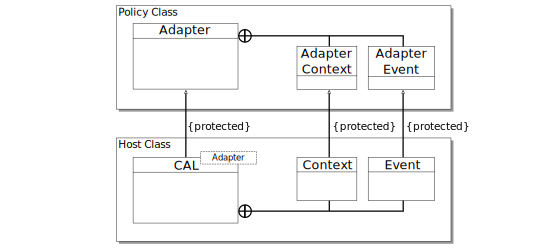
\includegraphics[width=\textwidth]{graphics/40_cal_uml}
  \caption{CAL implemented through policy based design. The adapter is
    configured by a template argument at compile-time. The CAL defines
    the context, event and communication interface. The adapter
    implements the determined interface of the CAL and the adapter-specific
    context and event classes.}
  \label{fig:cal_uml}
\end{figure}

\noindent The CAL provides all communication methods discussed in
Section~\ref{sec:des:p2p} and~\ref{sec:cal_collective} and context
creation methods discussed in Section~\ref{sec:cal_context}. The
communication policy implements all methods required by the adapter
definition that were discussed in
Section~\ref{sec:impl:policy_interface}.



%%%%%%%%%%%%%%%%%%%%%%%%%%%%%%%%%%%%%%%%%%%%%%%%%%%%%%%%%%%%%%%%%%%%%%%%%%%%%%%%
%                                                                              %
% POLICY INTERFACE                                                             %
%                                                                              %
%%%%%%%%%%%%%%%%%%%%%%%%%%%%%%%%%%%%%%%%%%%%%%%%%%%%%%%%%%%%%%%%%%%%%%%%%%%%%%%%
% Checked
\subsection{Communication Policy interface}
\label{sec:impl:policy_interface}
An adapter needs to implement the policy interface determined by the
CAL.  The interface was inspired by the sophisticated MPI language
binding for~C~\cite{ref:mpi_c_binding}. Therefore, it is implemented
on a rather low level of abstraction to provide the most possible
flexibility.  A subset of adapter methods was chosen to illustrate
the interface. A full listing of all methods should be retrieved from
the source code documentation.

\begin{itemize}

\item Point-to-Point Operation

  \begin{minipage}[t]{\textwidth} 
    \begin{lstlisting}[language=C++, breaklines=false, label={}]
// Adapter Method      
template <typename T_Data, T_Context>      
Event asyncSendData(const T_Data* data,      
                    const unsigned sendCount
                    const VAddr destination,
                    const T_Context context,
                    const unsigned tag); 
    \end{lstlisting}
    \end{minipage}
    
\item Collective Operation
  
  \begin{minipage}[t]{\textwidth} 
    \begin{lstlisting}[language=C++, breaklines=false, label={}]
// Adapter Method      
template <typename T_Data, T_Context>      
void gather(const T_Data* sendData,
            const unsigned sendCount,
            const T_Data* recvData,
            const unsigned recvCount,
            const VAddr root,
            const T_Context context);
    \end{lstlisting}
    \end{minipage}

\item Grouping
  
  \begin{minipage}[t]{\textwidth} 
    \begin{lstlisting}[language=C++, breaklines=false, label={}]
// Adapter Method
template <typename T_Context>      
T_Context createContext(const std::vector<VAddr> vAddrs,
                        const T_Context oldContext);
    \end{lstlisting}
    \end{minipage}
  
\end{itemize}

\noindent The adapter interface only provides a subset of operations
known from MPI or other communication libraries.  Most of these
operations were necessary during the implementation of the system or
used in example applications. Extending the adapter interface with
more operations is left as future work.


% Addressing of peers
% Checked
\subsection{Mapping to Virtual Addresses}
\label{sec:impl:vaddr}
Chapter~\ref{sec:design} established the requirement for an unified address
space to uniquely address peers in a context. The design decision was
focused on simplicity. Therefore, the address space for the
virtual addresses is in the range of natural numbers from zero to the
number of peers in a context minus one. A adapter needs to map its
own address space into the virtual address space. An example for such a
mapping is provided in Section~\ref{sec:cal_mpi_adapter}.


% Description Communication operations
% Checked
\subsection{CAL Data Object Interface}
All communication methods are able to transmit data objects of an
arbitrary data type defined by the template argument \cpp{T_Data}. The
data object needs to provide a pointer to the memory location where
the data is stored and the number of data elements to transmit.  The
method \cpp{data()} must return the memory pointer and the method
\cpp{size()} the number of elements of the data. C++ Containers of the
STL such as \cpp{std::vector} and \cpp{std::array}~\cite{ref:vector,
  ref:array} already provide these methods. Therefore, data can be
easily encapsulated into these containers. The following listing shows
the implementation of the \cpp{asyncSend()} method of the CAL. It
shows the usage of the discussed data object interface.  The object
\cpp{sendData} with data type \cpp{T_Data} must provide both functions
required by the data object interface. Utilizing \cpp{sendData.data()}
and \cpp{sendData.size()} fulfills the interface requirements of the
communication policy stated in
Section~\ref{sec:impl:policy_interface}.

%caption={},

\begin{minipage}[t]{\textwidth} 
  \begin{lstlisting}[language=C++, breaklines=false,  label={lst:cal_async_send}, caption={Data objects of the template data type \cpp{T\_Data} must provide the methods \cpp{data()} and \cpp{size()} which need to offer the memory pointer and the number of elements.}]
// Communication Abstraction Layer Method
template <typename T_Data>
Event asyncSend(const VAddr destVAddr, 
                const Tag tag, 
                const Context context, 
                const T_Data& sendData){

  return Event(
    CommunicationPolicy::asyncSendData(
      sendData.data(),
      sendData.size(), 
      destVAddr, 
      context, 
      tag
      
    )
      
  );

}
\end{lstlisting}
\end{minipage}

% Description Communication operations
% Checked
\subsection{Reduce Operation Interface}
The CAL reduce operation uses a binary operator to reduce a set of objects
of several peers. The C++ STL already provides a handfull of binary
functions in the \emph{functional} header such as \cpp{std::plus},
\cpp{std::multiplies} or \cpp{std::minus}
\cite{ref:functional}. Functions that are not provided by the STL can
be easily created with a C++ struct or class that overloads the
parenthesis operator. The following listing shows such a struct for
the maximum operator.

\begin{minipage}[t]{\textwidth} 
\begin{lstlisting}[language=C++, breaklines=false, caption={\ }, label={lst:binary_function}, caption={Implementation of the binary operator maximum. These kind of binary operators can be used for the CAL reduce operation.}]
template<typename T_Data>
struct maximum : public std::binary_function<T_Data, T_Data, T_Data> {

  // Parenthesis operator overloaded with binary operator for maximum
  const T_Data& operator()(const T_Data& x, const T_Data& y) const {
    return x < y? y : x;

  }

};
\end{lstlisting}
\end{minipage}%

\noindent An adapter that implements the reduce operation has to
ensure that it can handle binary operators.  There may exist cases in
which the C++ binary operator has to be transformed to an
adapter-specific one.  In these cases, the tranformation logic needs
to be implemented inside the adapter class.
Section~\ref{sec:bin_operator} discusses the transformation of binary
operators by the MPI adapter.

%%%%%%%%%%%%%%%%%%%%%%%%%%%%%%%%%%%%%%%%%%%%%%%%%%%%%%%%%%%%%%%%%%%%%%%%%%%%%%%%
%                                                                              %
% MPI ADAPTER                                                                  %
%                                                                              %
%%%%%%%%%%%%%%%%%%%%%%%%%%%%%%%%%%%%%%%%%%%%%%%%%%%%%%%%%%%%%%%%%%%%%%%%%%%%%%%%
% Checked
\section{The MPI Adapter as Reference Adapter Implementation}
\label{sec:cal_mpi_adapter}

A reference adapter is presented to provide an insight into the
development of an adapter and to provide hints on parts of the adapter
development that should be considered carefully. Furthermore, the
description provides a guideline for the implementation of additional
adapter classes.

The reference adapter implementation is based on MPI as existing
communication library. The adapter acts as a translation or mapping
from the CAL interface to the MPI interface.  MPI (Section
\ref{sec:mpi}) was chosen because it already provides a lot of
functionality required by the CAL interface without any further
effort. Additionally, it is available on wide range of computing
systems and can be used for free by open source implementations. This
section will utilize very MPI specific vocabulary. It is assumed
that the reader has a basic knowledge on MPI terminology.

The instantiation of a CAL object configured to use the MPI adapter
leads to an initialization of the MPI adapter. This initialization
step creates the initial global context by grouping all peers of
\cpp{MPI\_COMM\_WORLD}.  Furthermore, a mapping from MPI ranks to
virtual addresses for the global context is created in the
\cpp{vAddrMap}.  With respect to the definition of virtual addresses
in Section~\ref{sec:impl:vaddr}, the initial \cpp{vAddrMap} contains a
one-to-one mapping from virtual addresses in the global context to MPI
ranks in the \cpp{MPI\_COMM\_WORLD}.  The global context and each
derived context are mapped to MPI Communicators through a map data
structure called the \cpp{contextMap}.

%\todo{implement Boost::mpi adapter}

The MPI C language binding is used inside the adapter to address the
message passing interface.  It provides the most general interface to
MPI and can be integrated into a C++ environment.  This MPI interface
is very similar to the adapter interface. Therefore, the
implementation of the adapter interface through MPI routines is not
very complex. Nevertheless, the following listing shows that the
\cpp{asyncSendData} method does not only forward the function call to
the MPI communication method \cpp{MPI_Issend}.  But it also translates
the virtual address \cpp{destination} of the peer to the rank of the
MPI process through the \cpp{vAddrMap} at line~\ref{line:vAddrMap}.
Furthermore, it performs a translation of the context to the MPI
communicator in line~\ref{line:contextMap} through
the~\cpp{contextMap}. Finally, it converts the data type~\cpp{T_Data}
to an MPI data type in line~\ref{line:mpi_datatype}.  The conversion
of data types will be discussed in detail in
Section~\ref{sec:data_type_conversion}.

\begin{minipage}[t]{\textwidth} 
\begin{lstlisting}[language=C++, breaklines=false, caption={Communication method for non-blocking sending of data. The virtual address of the destination is translated to its MPI rank. The context is translated to an MPI communicator and the template data type \cpp{T\_Data} is translated to an MPI data type. The communication operation is finally performed by MPI.}, label={lst:adapter_send}, escapechar=|]
// Adapter Method
template <typename T_Data, typename T_Context>      
Event asyncSendData(const T_data* const data, 
                    const unsigned count, 
                    const Vaddr destination, 
                    const T_Context context, 
                    const unsigned msgType){    

  // Translation of vaddr to rank
  int destRank      = vAddrMap[context][destVaddr];|\label{line:vAddrMap}|

  // Translation of context to MPI Communicator
  MPI_Comm comm     = contextMap[context];|\label{line:contextMap}|

  // Conversion from T_Data to MPI data type
  MPI_Datatype type = ToMPIDatatype<T_Data>::type;|\label{line:mpi_datatype}|

  // MPI specific send operation                                                                            
  MPI_Request request; 
  MPI_Issend(const_cast<T_Data*>(data), 
             count, 
             type,
             destRank, 
             msgType,
             comm,
             &request);

  // Create and return event
  return Event(request);                                                                                                       

}  
\end{lstlisting}
\end{minipage}

\noindent The remaining adapter methods are implemented in a similar
manner, except for the reduce operation. Since the CAL interface
accepts arbitrary binary operators for reducing data, the MPI adapter
must be able to handle these
operators. The following Section~\ref{sec:bin_operator} covers the conversion of C++
binary operators to operators that are utilized in MPI.

%%%%%%%%%%%%%%%%%%%%%%%%%%%%%%%%%%%%%%%%%%%%%%%%%%%%%%%%%%%%%%%%%%%%%%%%%%%%%%%%
%                                                                              %
% BINARY OPERATOR                                                              %
%                                                                              %
%%%%%%%%%%%%%%%%%%%%%%%%%%%%%%%%%%%%%%%%%%%%%%%%%%%%%%%%%%%%%%%%%%%%%%%%%%%%%%%%
% Checked
\subsection{Binary Operator}
\label{sec:bin_operator}

MPI provides built-in support for binary operations by two
approaches. The simplest approach is the direct usage of predefined
binary MPI operators~\cite{ref:mpi_bin_op}. But, since the system user
should not utilize MPI operators directly, the CAL could wrap all
available MPI operators in a struct of static const expressions like
shown in Listing~\ref{lst:mpi_bin}.  The CAL could forward these
structs to the user of the system and the user could select from these
binary operators.  For example, a reduction by accumulation would use
the \cpp{BinaryOperations::SUM} operator.

\begin{minipage}[t]{\textwidth} 
\begin{lstlisting}[language=C++, caption={A subset of binary operators derived by transforming MPI operations to static const expressions. }, label=lst:mpi_bin]
struct BinaryOperations { 
  static constexpr BinaryOperation MAX = MPI_MAX; 
  static constexpr BinaryOperation MIN = MPI_MIN; 
  static constexpr BinaryOperation SUM = MPI_SUM; 
  static constexpr BinaryOperation PROD = MPI_PROD; 

};
\end{lstlisting}
\end{minipage}


\noindent The downside of this approach is, that only twelve predefined
operators exist, which restricts the application to this limited set of
operators. MPI provides the possibility to create abitrary
binary operators with the \cpp{MPI\_Op\_create} function.  The source
code for transforming abitrary binary operators to binary MPI
operators was taken from the boost::mpi project
\cite{ref:boost_mpi} and was adapted for the needs of the MPI adapter.
The following listing shows the transformation of the binary C++
operator \cpp{op} from type \cpp{T\_BinaryOperation} with data type
\cpp{T\_Data} to \cpp{MPIoperator} from type \cpp{MPI\_Op}.  After the
transformation, the MPI operator can be retrieved by and used by all
MPI routines that are using binary operators through
\cpp{MPIOperator.getOperator()}.

\begin{minipage}[t]{\textwidth} 
\begin{lstlisting}[language=C++, caption={ }, label=lst:mpi_bin2]
// Binary C++ operator
T_BinaryOperator op;  
  
// Transformation of binary operator
toMPIOperator<T_Data, T_BinaryOperator> MPIOperator(op);

// Retrieve binary MPI operator
MPIOperator.getOperator()
\end{lstlisting}
\end{minipage}

\noindent The second approach is substantially more flexible as the
first one. Thus, it was selected to implement binary operations for the
MPI adapter.

%%%%%%%%%%%%%%%%%%%%%%%%%%%%%%%%%%%%%%%%%%%%%%%%%%%%%%%%%%%%%%%%%%%%%%%%%%%%%%%%
%                                                                              %
% DATA TYPE CONVERSION                                                         %
%                                                                              %
%%%%%%%%%%%%%%%%%%%%%%%%%%%%%%%%%%%%%%%%%%%%%%%%%%%%%%%%%%%%%%%%%%%%%%%%%%%%%%%%
% Checked
\subsection{Data Type Conversion}
\label{sec:data_type_conversion}
On the one hand, MPI predefines primitive data types, but on the
other hand also provides the possibility to define data structures
based upon sequences of the MPI primitive data types. These user
defined data structures are called derived data types. Usually,
primitive data types are contiguous, which means that they form a
solid block of memory with no gaps in between. However, derived data
types allow you to specify non-contiguous data in a comfortable manner
and to treat it as though it was contiguous.  Therefore, more complex
data types (e.g linked lists or maps) can be transformed into derived
data types. The exchange of complex data types was not necessary in
the development of the system based on examples of Section
\ref{sec:gol_imp}. Therefore, the implementation was focused on the
transformation of primitive data types.  Nevertheless, a
transformation is available in the boost::mpi \cite{ref:boost_mpi}
implementation. Thus switching to boost::mpi or adopting their source
code would solve this problem without any further effort.

The primitive C++ data types can be mapped directly to primitive MPI
data types. Based on the fact that MPI data types are defined as C macros,
a C++ data type needs to be converted to an integer number. The
conversion is implemented by the concept of type traits
\cite{ref:type_trait}.  Type traits are classes that obtain
characteristics of types in the form of compile-time constant values.

The type trait is responsible for the transformation of primitive C++
data types to primitive MPI data types.  In
Listing~\ref{lst:mpi_trait1} a template struct defines the default
behavior of the type trait. The struct defines a static const
expression \cpp{type}, which is set to a fixed MPI data type. The
template argument \cpp{T_Data} is the primitive C++ data type that
should be transformed. The default struct will transform arbitrary
data types \cpp{T_Data} to the \cpp{MPI\_INT} data type. The MPI data
type of \cpp{T_Data} can be retrieved by
\cpp{ToMPIDatatype<T_Data>::type}.

\begin{minipage}[t]{\textwidth} 
\begin{lstlisting}[language=C++, label=lst:mpi_trait1, caption={A templated struct defines the default behavior of the type trait. It will transform arbitrary data types \cpp{T\_Data} to the MPI\_INT data type if no other type trait is defined}]
  template<typename T_Data> 
  struct ToMpiDatatype { 

    static constexpr MPI_Datatype type = MPI_INT; 

  };
\end{lstlisting}
\end{minipage}

\noindent The template in Listing~\ref{lst:mpi_trait2} is an explicit
specialization of the default template in
Listing~\ref{lst:mpi_trait1}. In this case, a specialization for the
C++ data type \cpp{char}, which will be transformed to the
\cpp{MPI\_CHAR} data type.  Thus, each transformation of a primitive
C++ data type needs to be defined by its own specialization template.

\begin{minipage}[t]{\textwidth} 
  \begin{lstlisting}[language=C++, label=lst:mpi_trait2, caption={A specialization of the default type trait for the C++ data type \cpp{char}. It transforms \cpp{char} to the \cpp{MPI\_CHAR} data type.}]
  template<>
  struct ToMPIDatatypes<char> { 

    static constexpr MPI_Datatype type = MPI_CHAR; 

  };
\end{lstlisting}
\end{minipage}

\noindent The communication operations within the adapter use the
type traits to transform the data types of the input and output data
by querying the type trait. The following listing provides an example
for the conversion of the C++ data type \cpp{char}.

\begin{minipage}[t]{\textwidth} 
\begin{lstlisting}[language=C++, label=lst:mpi_trait3]
  MPI_Datatype type = ToMPIDataType<char>::type;
\end{lstlisting}
\end{minipage}

%%%%%%%%%%%%%%%%%%%%%%%%%%%%%%%%%%%%%%%%%%%%%%%%%%%%%%%%%%%%%%%%%%%%%%%%%%%%%%%%
%                                                                              %
% CONTEXT EVENT MPI ADAPTER                                                    %
%                                                                              %
%%%%%%%%%%%%%%%%%%%%%%%%%%%%%%%%%%%%%%%%%%%%%%%%%%%%%%%%%%%%%%%%%%%%%%%%%%%%%%%%
% Checked
\subsection{MPI Adapter Specific Event Implementation}
The MPI adapter-specific \cpp{Event} utilizes the MPI functions
\cpp{MPI\_Wait} and \cpp{MPI\_Test} to test non-blocking operations
for termination. In MPI, a non-blocking function returns a request
object, which is the handle to verify if a the function
terminated. The following listing shows the \cpp{Event} implementation
of the MPI adapter.  The \cpp{wait()} method is implemented by using
\cpp{MPI\_Wait} on the request. The \cpp{ready()} method uses
\cpp{MPI\_Test} to check if the non-blocking function terminated.

\begin{minipage}[t]{\textwidth} 
  \begin{lstlisting}[language=C++, label=lst:mpi_event, caption={MPI adapter-specific \cpp{Event} implementation. Non-blocking MPI operations can be handled by an \cpp{MPI\_Request} object. The \cpp{wait()} method waits until the communication operation terminated
    with \cpp{MPI\_Wait}. The \cpp{ready()} method checks if the communication operation terminated with \cpp{MPI\_Test}.}]
class Event {
  public:

  Event(MPI_Request request) : request(request){
    
  }
  
  ~Event(){
    
  }

  void wait(){
    MPI_Status status;
    MPI_Wait(&request, &status);
    
  }

  bool ready(){
    int flag = 0;
    MPI_Status status;
    MPI_Test(&request, &flag, &status);
    return bool(flag);
    
  }
  
  private:
  
  MPI_Request request;
  
};  
\end{lstlisting}
\end{minipage}

%%%%%%%%%%%%%%%%%%%%%%%%%%%%%%%%%%%%%%%%%%%%%%%%%%%%%%%%%%%%%%%%%%%%%%%%%%%%%%%%
%                                                                              %
% GRAPH IMPLEMENTATION                                                         %
%                                                                              %
%%%%%%%%%%%%%%%%%%%%%%%%%%%%%%%%%%%%%%%%%%%%%%%%%%%%%%%%%%%%%%%%%%%%%%%%%%%%%%%%
% Checked
\section{Graph Based on the Boost Graph Library}
\label{sec:impl:graph}
Section \ref{sec:graph} introduced a graph interface.  This graph
interface is implemented on basis of an existing graph library as
back-end. A wide range of graph libraries such as \cite{ref:lemon,
  ref:boost_bgl, ref:igraph, ref:ogdf} were considered as back-end
libraries.  However, since, the Boost project is closely related to
the STL, the \emph{Boost Graph Library} \cite{ref:boost_bgl} (BGL) was
selected as graph back-end library.  While the BGL provides a powerful
and complex interface with wide range of graph algorithms, just a small subset of
this functionality is really necessary.

Therefore, the BGL is wrapped inside a graph class providing common
graph functionality which simplifies the BGL interface.  The graph
class provides all methods discussed in design Section
\ref{sec:graph}, but the methods are internally handled by the BGL.


%%%%%%%%%%%%%%%%%%%%%%%%%%%%%%%%%%%%%%%%%%%%%%%%%%%%%%%%%%%%%%%%%%%%%%%%%%%%%%%%
%                                                                              %
% PROPERTIES                                                                   %
%                                                                              %
%%%%%%%%%%%%%%%%%%%%%%%%%%%%%%%%%%%%%%%%%%%%%%%%%%%%%%%%%%%%%%%%%%%%%%%%%%%%%%%%
% Checked
\subsection{Vertices Annotated by Properties}

A graph in the BGL can be anotated by properties. These objects are
used to describe vertices and edges with simulation-specific
information, as it was discussed in Section~\ref{sec:graph}. Vertices
and edges are provided with properties at compile-time through a
template parameter.  The BGL refers to vertices and edges by indices
of integer numbers, whereby properties of this vertices can be queried
from so called property maps.  The graph connects these indices with
its properties to create a vertex and edge description.

The implementation of a property is a struct or a class with arbitrary
content. It needs to provide an \cpp{id} member variable or inherit
it from \cpp{SimpleProperty}. This \cpp{id} is used to create an internal
mapping of the property to the vertex index of the BGL.  The 
simplest property is a struct only containing the \cpp{id}, as
presented in Listing \ref{lst:property}. This property is predefined
in the graph header. It is used as default property when the graph is not
configured by a certain property.

\begin{minipage}[t]{\textwidth} 
\begin{lstlisting}[language=C++, label=lst:property, caption={Predefined property within the graph class which only provides an id member variable. This property can be used a skeleton for further property implementations. }]
struct SimpleProperty {

    SimpleProperty() : id(0) {

    }
    
    SimpleProperty(ID id) : id(id) {

    }

    // Vertex id refers to BGL vertex index
    unsigned id;
    
};
\end{lstlisting}
\end{minipage}

\noindent Requesting the vertices of the graph returns a vector with
all vertices of the graph. However, that vector contains all vertex
properties in the context of the BGL. Each of these properties
represents a mapping to the internal BGL graph. This mapping is
transparent to the system user. Hence, the user does not have to care
about it.

%%%%%%%%%%%%%%%%%%%%%%%%%%%%%%%%%%%%%%%%%%%%%%%%%%%%%%%%%%%%%%%%%%%%%%%%%%%%%%%%
%                                                                              %
% CREATION OF A GRAPH                                                          %
%                                                                              %
%%%%%%%%%%%%%%%%%%%%%%%%%%%%%%%%%%%%%%%%%%%%%%%%%%%%%%%%%%%%%%%%%%%%%%%%%%%%%%%%
% Checked
\subsection{Creation of a Graph}
A graph is created by a vector of edge descriptors and a vector of
corresponding vertices. An edge descriptor is the tuple of source
vertex, destination vertex and the connecting edge. The vector of edge
descriptors can also be generated by a graph
generator. Listing~\ref{lst:graph} demonstrates the creation of a graph from
a hypercube topology with three dimensions.

\begin{minipage}[t]{\textwidth} 
\begin{lstlisting}[language=C++, label=lst:graph, caption={Generation of a three-dimensional hypercube graph. }]
// Definition of EdgeDescriptor
typedef std::tuple<Vertex, Vertex, Edge> EDesc;
const unsigned nDimensions = 3;

// Create vertex and edge vectors
std::vector<Vertex> vertices;
std::vector<EDesc> edges = Topology::hypercube<Graph>(nDimensions, vertices);

// Create graph by edges and vertices
Graph graph(edges, vertices);

\end{lstlisting}
\end{minipage}

\noindent Figure \ref{fig:topologies} depicts a set of implemented
generators of commonly used graph topologies.  This set of generators
covers fully connected topology, star topology, n-dimensional grid
topology, and n-dimensional hypercube topology.  These generators are
parametrizable by the number of vertices and/or dimension.
Communicaton topologies are usually implemented from the scratch, but
these topology generator functions have the advantage that they can be
reused in different applications with same communication topology.

\begin{figure}[H]
  \centering
  \includegraphics[width=\textwidth]{graphics/40_topologies}
  \caption{Set of already implemented graph generators.}
  \label{fig:topologies}
\end{figure}

%%%%%%%%%%%%%%%%%%%%%%%%%%%%%%%%%%%%%%%%%%%%%%%%%%%%%%%%%%%%%%%%%%%%%%%%%%%%%%%%
%                                                                              %
% CREATION OF SUBGRAPHS                                                        %
%                                                                              %
%%%%%%%%%%%%%%%%%%%%%%%%%%%%%%%%%%%%%%%%%%%%%%%%%%%%%%%%%%%%%%%%%%%%%%%%%%%%%%%%
% Checked
\subsection{Creation of a Subgraph}
The creation of a subgraph plays an important role for collective
operations on a subset of graph vertices by the GVON
(Section~\ref{sec:design:gvon_collectives}). A subgraph is created
from a graph by selecting a subset of its vertices.  Subgraph creation is
utilized as an equivalent to the creation of sub contexts in the
CAL. Collective operations on this subgraph only consider vertices
within this subgraph. The BGL provides already built-in support for
subgraphs. The following listing demonstrates the creation of a
subgraph.

\begin{minipage}[t]{\textwidth} 
\begin{lstlisting}[language=C++, label=lst:subgraph]
  // Creation of a subgraph
  Graph& subGraph = graph.createSubGraph(subGraphVertices);
  
\end{lstlisting}
\end{minipage}

\noindent A created subgraph is linked to its supergraph, whereby each
supergraph holds a list of its subgraphs. The connection of super- and
subgraph is important for the context creation for collective
operations in Section~\ref{sec:gvon_impl}, because the announcement of
a subgraph considers first of all the context of the
supergraph. Figure \ref{fig:subgraph_creation} depicts the creation of
a two-dimensional hypercube subgraph from a three-dimensional
hypercube graph.

\begin{figure}[H]
  \centering
  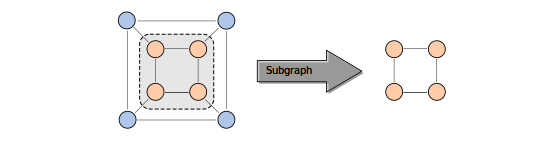
\includegraphics[width=\textwidth]{graphics/40_subgraph_creation}
  \caption{Inner vertices of a three-dimensional hypercube graph are 
  transformed to a two-dimensional hypercube subgraph. Both graphs
  stay in connection by the BGL.}
  \label{fig:subgraph_creation}
\end{figure}

%%%%%%%%%%%%%%%%%%%%%%%%%%%%%%%%%%%%%%%%%%%%%%%%%%%%%%%%%%%%%%%%%%%%%%%%%%%%%%%%
%                                                                              %
% GRAPH BASED VIRTUAL OVERLAY NETWORK                                          %
%                                                                              %
%%%%%%%%%%%%%%%%%%%%%%%%%%%%%%%%%%%%%%%%%%%%%%%%%%%%%%%%%%%%%%%%%%%%%%%%%%%%%%%%
% Checked
\section{GVON Implementation}
\label{sec:gvon_impl}
The GVON was introduced as a combination
of the graph and CAL. This combination is the connection of graph and CAL
through mappings. These mappings are core components of the GVON and are
constructed by the announcement process. The announcement process
implementation is discussed in Section~\ref{sec:announcement_impl}. In
the following, each map provided by the GVON is described:

\begin{itemize}
\item [] The \cpp{vertexMap} is a mapping from a vertex to the virtual
address of its host.  This map is used for all methods
that need to resolve the host of a vertex.

\begin{minipage}[t]{\textwidth} 
\begin{lstlisting}[language=C++, label=lst:mapping1]
std::map<Graph, std::map<Vertex, VAddr>> vertexMap;
\end{lstlisting}
\end{minipage}


\item [] The \cpp{graphMap} is a mapping from a graph to its related
  context. This context is created exclusively for this graph in the
  announcement process.  This map is important, since only the hosts
  of a graph are able to communicate on basis of this graph.

  \begin{minipage}[t]{\textwidth} 
    \begin{lstlisting}[language=C++, label=lst:mapping2]
std::map<Graph, Context> graphMap;
    \end{lstlisting}
    \end{minipage}


\end{itemize}
%% \paragraph*{}
%% \todo{What is the peerMap used for ?}
%% \noindent The \cpp{peerMap} is kind of a reverse mapping of the
%% \cpp{vertexMap}.  This map is a mapping from peers to its hosted
%% vertices for a particular graph.
%% \begin{lstlisting}[language=C++, label=lst:mapping3]
%% std::map<Graph, std::map<VAddr, std::vector<Vertex>> > peerMap 
%% \end{lstlisting}

\noindent Listing \ref{lst:comm_gvon} shows the \cpp{asyncSend} method of the
GVON. The vertex is translated to its host's virtual address in line
\ref{line:gvon_async_send1}. The graph is translated to its context
in line \ref{line:gvon_async_send2}.

\begin{minipage}[t]{\textwidth} 
\begin{lstlisting}[language=C++, label=lst:comm_gvon, caption={The \cpp{vertexMap} is used to translate vertices to virtual addresses and \cpp{graphMap} is used to translate graphs to contexts. The communication operation is performed by the the CAL.}, escapechar=| ]
// Graph-Based Virtual Overlay Network Operation  
template <typename T_Data>
Event asyncSend(Graph& graph, 
                const Vertex destVertex, 
                const Edge edge, 
                const T_Data& data){ 

  // Retrieve host virtual address of destVertex in graph
  VAddr destVAddr = vertexMap[graph][destVertex];|\label{line:gvon_async_send1}|

  // Retrieve context of the graph
  Context context = contextMap[graph];|\label{line:gvon_async_send2}|

  // Use CAL to send data
  return cal.asyncSend(destVAddr, edge.id, context, data);

}
\end{lstlisting}
\end{minipage}

\noindent Collective operations also utilize the GVON mappings, but their
implementations are far more complex. These collective implementations will be
discussed in detail in Section~\ref{sec:gvon_collective}.


%%%%%%%%%%%%%%%%%%%%%%%%%%%%%%%%%%%%%%%%%%%%%%%%%%%%%%%%%%%%%%%%%%%%%%%%%%%%%%%%
%                                                                              %
% ANNOUNCEMENT PROCESS                                                         % 
%                                                                              %
%%%%%%%%%%%%%%%%%%%%%%%%%%%%%%%%%%%%%%%%%%%%%%%%%%%%%%%%%%%%%%%%%%%%%%%%%%%%%%%%
% Checked
\subsection{Announcement Process of Graphs}
\label{sec:announcement_impl}

Peers that want to host vertices need to announce these vertices.
Therefore, the GVON Interface provides an announcement method for the
construction of two mappings. First, a mapping from vertices to peers
of a context in the \cpp{vertexMap}. Second, a mapping from graphs to
new created contexts in the \cpp{graphMap}.  The method takes a pair
of a graph and a vector of vertices as input arguments.  It is a
collective operation of all the peers that want to take part on the
communication of this graph.

These peers need to create an exclusive context for
themselves, which only contains hosts of the graph that will be
announced.  To that end, the most general context of the hosts, possibly
including more peers, has to be determined.  The overall most general
context is the global context of all peers in the network, but in some
cases there exists also a context with less peers.  This is either the
context of the graph or the context of the supergraph, if these graphs
were already announced.

This most general context is used to gather the number of hosted
vertices of each host and to create a new context that only contains
peers which host at least one vertex. The graph is mapped to this new
context in the \cpp{graphMap}.

Furthermore, this new context is used for announcing the hosted
vertices of each host through an \cpp{allGather} operation, such that
each host can update its \cpp{vertexMap} for this context.

%%%%%%%%%%%%%%%%%%%%%%%%%%%%%%%%%%%%%%%%%%%%%%%%%%%%%%%%%%%%%%%%%%%%%%%%%%%%%%%%
%                                                                              %
% COLLECVITE OPERATIONS LOCALLY                                                %
%                                                                              %
%%%%%%%%%%%%%%%%%%%%%%%%%%%%%%%%%%%%%%%%%%%%%%%%%%%%%%%%%%%%%%%%%%%%%%%%%%%%%%%%
% Checked
\subsection{Collective Operations on Graphs}
\label{sec:gvon_collective}

Since hosts manage potentially more than a single vertex, a host has
to perform the collective operation at first locally for its hosted
vertices. This means, that the data of each hosted vertex has to be
collected locally before the collective operation of the CAL can be
performed. The fact that data objects can have arbitrary data types
increases the difficulty of the implementation of these collective
operations.  In the following, the collector of a GVON collective is
described:

\begin{itemize}
\item []
  The collector is a templated \cpp{static} object from type
  \cpp{std::vector<T_Data>}.  The data of the hosted vertices is
  collected in a collector object until all hosted vertices of this
  host have terminated their collective operation. Such a collector
  will be created for each data type \cpp{T_Data}.

  \begin{minipage}[t]{\textwidth} 
  \begin{lstlisting}[language=C++, label=lst:static_collective]
// Type dependent instanciation of the collector
static std::vector<T_Data> collector;
  \end{lstlisting}
  \end{minipage}

\item [] Since in some cases the resulted data is received by a root vertex, the host of
the root vertex stores the receive object pointer.

\begin{minipage}[t]{\textwidth} 
\begin{lstlisting}[language=C++, label=lst:root]
// Receive object pointer of root host
static T_Data* rootRecvData;
\end{lstlisting}
\end{minipage}


\item [] Each call of a collective operation is collecting the vertex
  data of the calling host in the collector.  In the case a host is
  calling the operation with the root vertex, the receive pointer of
  the root vertex is stored.

  
\begin{minipage}[t]{\textwidth}
  \begin{lstlisting}[language=C++, label=lst:collecting]
// Collection of vertex data
collector.push_back(vertexData);
  \end{lstlisting}
  \end{minipage}

\end{itemize}

%A peer could try to mix the execution of collective operations of
%several graphs. But, it is only one collective per pair of a graph and
%a vertex allowed concurrently. To ensure that, the amount of already
%executed collective operations per vertex on a graph is counted.  Is
%this count at the beginning of a collective greater than zero, then
%the collective execution is aborted by an exception.

\noindent If the last data object is collected, the
operation is executed locally for each host and its result is forwarded to the CAL
interface. The CAL executes the collective operation among all
other hosts of the graph and returns the result. For collectives such as
\cpp{gather}, the resulting data is reordered such that the GVON returns the
data in ascending vertex id order. Finally, the result is written to the receive
pointer of the root vertex.


%%%%%%%%%%%%%%%%%%%%%%%%%%%%%%%%%%%%%%%%%%%%%%%%%%%%%%%%%%%%%%%%%%%%%%%%%%%%%%%%
%                                                                              %
% GAME OF LIFE IMPLEMENTATION                                                  %
%                                                                              %
%%%%%%%%%%%%%%%%%%%%%%%%%%%%%%%%%%%%%%%%%%%%%%%%%%%%%%%%%%%%%%%%%%%%%%%%%%%%%%%%

\section{Implementing a Game of Life}
\label{sec:impl:gol}
The Game of Life simulation was implemented to show the developed
system in a real world scenario. The set of implemented rules based on
\cite{ref:gol_rules} is listed in the following:

\begin{enumerate}
\item Any live cell with fewer than two live neighbors dies, caused by underpopulation.
\item Any live cell with two or three live neighbors lives on to the next generation.
\item Any live cell with more than three live neighbors dies, caused by overpopulation.
\item Any dead cell with exactly three live neighbors becomes a live cell, caused by reproduction.
\end{enumerate}

%%%%%%%%%%%%%%%%%%%%%%%%%%%%%%%%%%%%%%%%%%%%%%%%%%%%%%%%%%%%%%%%%%%%%%%%%%%%%%%%
%                                                                              %
% CONFIGURATION AND INITIALIZATION OF GOL                                      %
%                                                                              %
%%%%%%%%%%%%%%%%%%%%%%%%%%%%%%%%%%%%%%%%%%%%%%%%%%%%%%%%%%%%%%%%%%%%%%%%%%%%%%%%
% Checked
\subsection{Configuration and Initialization of Game of Life}
The following source code describes necessary steps to configure and
initialize the system before starting the communication of the
GoL. The source code uses the presented MPI adapter, GoL graph and
Cell property. It demonstrates the general program flow and can be the
foundation for other simulation applications.

\begin{enumerate}

\item \textbf{Configuration}
\begin{enumerate}

\item Configure the CAL
  
  The target system is a cluster providing MPI as communication
  library. Therefore, the CAL is configured by the reference MPI adapter
  described in Section~\ref{sec:cal_mpi_adapter}. The adapter provides
  type definitions for the virtual address, event and context that are
  necessary for later usage:

  \begin{minipage}[t]{\textwidth} 
  \begin{lstlisting}[language=C++, label=lst:conf_cal, caption={\ }]
// Configure CAL
typedef CommunicationPolicy::MPI                  Mpi;
typedef CommunicationAbstractionLayer<Mpi>        MpiCAL;
typedef typename MpiCAL::VAddr                    VAddr;
typedef typename MpiCAL::Event                    Event;
  \end{lstlisting}
  \end{minipage}

\item Configure the graph

  The graph is configured with the vertex property \cpp{Cell} 
  (Listing~\ref{lst:gol_cell}) and the edge property \cpp{SimpleProperty}. It
  provides type definitions for vertex and  edge:

  \begin{minipage}[t]{\textwidth} 
  \begin{lstlisting}[language=C++, label=lst:conf_graph, caption={\ }]
// Configure graph
typedef Graph<Cell, SimpleProperty>               GoLGraph;
typedef typename GoLGraph::Vertex                 Vertex;
typedef typename GoLGraph::Edge                   Edge;
  \end{lstlisting}
  \end{minipage}

  The \cpp{Cell} property contains the state information of a cell,
  and inherits the vertex id from \cpp{SimpleProperty}.  The following
  listing shows the source code of the \cpp{Cell} property.

  \begin{minipage}[t]{\textwidth} 
  \begin{lstlisting}[language=C++, label=lst:gol_cell, caption={\ }]
// Cell property    
struct Cell : public SimpleProperty { 

 Cell() : SimpleProperty(0), isAlive{{0}}, aliveNeighbors(0){ 
          
 }
        
 // Initialization of the cell
 Cell(ID id) : SimpleProperty(id), isAlive{{0}}), aliveNeighbors(0){ 
   unsigned random = rand() % 10000;
   if(random < 3125){ 
     isAlive[0] = 1;
     
   }
   
 }

 // State of the cell
 std::array<unsigned, 1> isAlive;

 // Number of alive neighbors
 unsigned aliveNeighbors;
 
};
  \end{lstlisting}
  \end{minipage}

\item Configure the GVON

  The GVON is configured by the previously configured \cpp{GoLGraph}
  and \cpp{MpiCAL}~(Listings~\ref{lst:conf_graph}~\ref{lst:conf_cal}).

  \begin{minipage}[t]{\textwidth} 
  \begin{lstlisting}[language=C++, label=lst:conf_gvon, caption={}]
// Configure GVON
typedef VirtualOverlayNetwork<GoLGraph, MpiCAL> GVON;
  \end{lstlisting}
  \end{minipage}

\end{enumerate}

\item \textbf{Initialization}
  \begin{enumerate}
  
  \item Create the graph object

    The graph is generated by the predefined graph generator for
    grids. The generator creates a two dimensional grid, where cells
    are connected to their vertical, horizontal and diagonal neighbors
    (Figure~\ref{fig:gol_modeling}).

    \begin{minipage}[t]{\textwidth} 
  \begin{lstlisting}[language=C++, label=lst:gol_generator_graph, caption={}]
// STL namespace
using namespace std;

// Type definitions
typedef typename GoLGraph::EdgeDescriptor EDesc;

// Generate GoL graph
vector<Vertex> vertices;
vector<EDesc> edges = Topology::grid<GoLGraph>(n, vertices);
GoLGraph graph (edges, vertices); 
  \end{lstlisting}
  \end{minipage}

\item Create the CAL and GVON objects

  \begin{minipage}[t]{\textwidth} 
  \begin{lstlisting}[language=C++, label=lst:, caption={}]
// Instantiate CAL and GVON
MpiCAL cal;
GVON gvon(cal);
  \end{lstlisting}
  \end{minipage}

\item Distribute the vertices

  The graph vertices are distributed in round-robin fashion, which
  is by far not the optimal vertex distribution method, but this is not the
  focus of this work.

  \begin{minipage}[t]{\textwidth} 
  \begin{lstlisting}[language=C++, label=lst:gol_distribution, caption={}]
// Distribution of vertices by round-robin
Context context = cal.getGlobalContext();
vector<Vertex> hostedVertices = Dist::roundrobin(context, graph);
  \end{lstlisting}
  \end{minipage}

  \noindent Figure
  \ref{fig:gol_mapping} shows two alternative vertex distributions
  methods.  In the first variant, hosted vertices are connected
  within the same host, since this reduces communication operations
  with other peers over a network.  In the second variant, every vertex is
  hosted by exactly one peer, representing a case where the graph
  represents exactly the communicating processes.

  \begin{figure}[H]
    \centering
    \includegraphics[width=\textwidth]{graphics/40_gol_mapping}
    \caption{Image detail of one section of the GoL world. Possible
      distributions of modeled GoL graph. On the left-hand side, a
      peer hosts a connected set of vertices. On the right-hand side,
      every peer hosts exactly one vertex.}
    \label{fig:gol_mapping}
  \end{figure}

  \noindent Possible distributions range from one host that hosts all
  vertices to the number of hosts where every host is responsible for
  a single vertex. Expanding this range for an execution of an
  application with more peers than available vertices offers an
  interesting case for fault tolerance and load balancing.  Additional
  peers could be used as backup peers, but this is left open for
  future work.  After distribution vertices, every peer announces its
  vertices to the GVON.

\item Announcement of the hosted vertices

  \begin{minipage}[t]{\textwidth} 
  \begin{lstlisting}[language=C++, label=lst:gol_announce, caption={}]
// Announcement of hosted vertices
gvon.announce(graph, hostedVertices);
  \end{lstlisting}
  \end{minipage}
  
  \end{enumerate}
\end{enumerate}

%%%%%%%%%%%%%%%%%%%%%%%%%%%%%%%%%%%%%%%%%%%%%%%%%%%%%%%%%%%%%%%%%%%%%%%%%%%%%%%%
%                                                                              %
% COMMUNICATION OF GAME OF LIFE                                                %
%                                                                              %
%%%%%%%%%%%%%%%%%%%%%%%%%%%%%%%%%%%%%%%%%%%%%%%%%%%%%%%%%%%%%%%%%%%%%%%%%%%%%%%%
% Checked
\subsection{Communication of Game of Life}
\label{sec:gol_imp}
Since the utilized GoL rules only require next-neighbor communication,
the GoL domain is modeled as a two-dimensional grid with diagonal
connections as shown in Figure~\ref{fig:gol_modeling}. Therefore, a
GoL cell is represented by a vertex and neighboring cells are
connected by edges. A cell has to communicate with its neighboring
cells to retrieve the neighboring cells states and to calculate its own
state for the next time-step.

In the following, the implementation of a single time-step of the GoL
is described. The communication between vertices of the GoL graph is
handled by the GVON. A host knows all its hosted vertices whose
communication it needs to manage. In the case of GoL, a host has to
exchange the state of its hosted cells with all neighboring cells.

First, each host sends the state of its cells to all neighboring
cells (Listing \ref{lst:gol_send}). The host retrieves the target
vertex of each outgoing edge for a hosted vertex from the graph. After that,
the state of the corresponding cell is transmitted to the target vertices
sequentially in non-blocking mode (Figure
\ref{fig:gol_communication}). Events of the send operation are
collected and checked later for termination.

\begin{minipage}[t]{\textwidth} 
\begin{lstlisting}[language=C++, label=lst:gol_send, caption={A host sends the cell state of its hosted vertices to all neighboring vertices. The information of neighboring vertices is retrieved from the graph. The cell states are send in the non-blocking variant.}]
// Send state to neighbor cells
for(Vertex myVertex : hostedVertices){
  for(std::pair<Vertex, Edge> outEdge : graph.getOutEdges(myVertex)){

    // Retrieve target vertex
    Vertex targetVertex = outEdge.first;
    Edge   edge         = outEdge.second;

    // Send cell state to neighboring cell
    events.push_back(
      gvon.asyncSend(graph, targetVertex, edge, myVertex.isAlive)
    );

  }

}
\end{lstlisting}
\end{minipage}

\noindent Figure \ref{fig:gol_communication} shows the sending process
of a host for each of its hosted vertices. The host queries the graph
for outgoing edges for each of its hosted vertices. The cell state of
a hosted vertex needs to be send to the target vertices of its outgoing
edges.

\begin{figure}[H]
  \centering
  \includegraphics[width=\textwidth]{graphics/40_gol_communication}
  \caption{Image detail of one section of the GoL world. A host sends
    the cell state of its hosted vertices to neighboring vertices.}
  \label{fig:gol_communication}
\end{figure}

\noindent As a second step, each host receives state information of
neighboring cells for each of its hosted vertices (Listing
\ref{lst:gol_recv}). The host queries the source vertex of incoming
edges of its hosted vertices from the graph. Afterwards, it receives
the state information from this neighboring source vertex.  The
receive operation is used in blocking mode to ensure that all peers
are synchronized afterwards.

\begin{minipage}[t]{\textwidth} 
\begin{lstlisting}[language=C++, label=lst:gol_recv, caption={A host receives the cell state of neighboring vertices of its hosted vertices. The information of neighboring vertices is retrieved from the graph. The cell states are received in the blocking variant to synchronize the hosts.}]
// Recv state from neighbor cells
for(Vertex myVertex : hostedVertices){
  for(std::pair<Vertex, Edge> inEdge : graph.getInEdges(myVertex)){

    // Retrieve source vertex
    Vertex sourceVertex = inEdge.first;
    Edge   edge         = inEdge.second;

    // Receive cell state of the neighboring cell    
    gvon.recv(graph, sourceVertex, edge, sourceVertex.isAlive);

    // Update number of living neighbors
    if(sourceVertex.isAlive[0]) { 
      myVertex.aliveNeighbors++;

  }

}
\end{lstlisting}
\end{minipage}



\noindent Once all send and receive operations terminated, the host
updates the cell states of its hosted vertices according to the introduced rules. Finally, the
state information of all cells is gathered by the root vertex (vertex
with id equal to zero) which prints it to the console for visualization (Listing
\ref{lst:gol_gather}). The next time-steps will repeat the
previous communication steps until the application is aborted or a
fixed number of time-steps is reached.

\begin{minipage}[t]{\textwidth} 
  \begin{lstlisting}[language=C++, label=lst:gol_gather, caption={The cell states of all vertices of the GoL graph is
    gathered by a host that hosts the root vertex.} ]
// Gather state by root vertex
for(Vertex myVertex: hostedVertices){
  gvon.gather(root, myVertex, graph, myVertex.isAlive, golGameField);

}
\end{lstlisting}
\end{minipage}


%%%%%%%%%%%%%%%%%%%%%%%%%%%%%%%%%%%%%%%%%%%%%%%%%%%%%%%%%%%%%%%%%%%%%%%%%%%%%%%%
%                                                                              %
% Implementation N-BODY                                                        %
%                                                                              %
%%%%%%%%%%%%%%%%%%%%%%%%%%%%%%%%%%%%%%%%%%%%%%%%%%%%%%%%%%%%%%%%%%%%%%%%%%%%%%%%
\section{Implementing a N-Body Simulation}
\label{sec:impl:nbody}


The implementation of the N-body simulation, discussed in Section
\ref{sec:design:nbody} is very similar to the GoL
implementation with respect to the GVON. Its implementation is
also split into three phases: configuration, initialization and
communication. The slight differences in implementation details are
described in the following enumeration:

\begin{enumerate}
\item \textbf{Configuration}

  The graph is annotated by the property \cpp{Particle}, containing
  information about the particle's mass, velocity, and location.

\item \textbf{Initialization}

  Since the chosen N-body algorithm is
  based on an all-to-all communication pattern, the communication
  dependencies are modeled as a fully connected graph.

\item \textbf{Communication}

  Every host sends particle information
  of its hosted vertices to adjacent vertices. In return, it receives
  particle information from all adjacent vertices. Since a vertex is
  adjacent to all other vertices, it sends to and receives from
  all other vertices.
\end{enumerate}

\noindent After each communication step, a host updates the state of
the particles of its hosted vertices.  The communication phase is
repeated for an arbitrary but fixed amount of time steps or until the simulation
execution is canceled.

The implemented N-body simulation is completely different from the
presented GoL implementation, but uses similar communication
concepts. Therefore, the source code responsible for communication in
the GoL simulation can be reused to implement this N-body simulation.



%%%%%%%%%%%%%%%%%%%%%%%%%%%%%%%%%%%%%%%%%%%%%%%%%%%%%%%%%%%%%%%%%%%%%%%%%%%%%%%%
%                                                                              %
% REDISTRIBUTION OF VERTICES                                                   %
%                                                                              %
%%%%%%%%%%%%%%%%%%%%%%%%%%%%%%%%%%%%%%%%%%%%%%%%%%%%%%%%%%%%%%%%%%%%%%%%%%%%%%%%
\section{Redistribution of Vertices}

The GVON provides explicit mappings from vertices to peers and from
graphs to contexts. These mappings can be modified dynamically at the
run-time of the simulation application.  To demonstrate that behavior
of the system, an occupation scenario, where a vertex is changing its
host is implemented. This is possible, since hosted vertices are not
bound statically to their hosts.

The scenario is the following: a host occupies or steals a vertex
from another host and henceforth hosts this vertex.  This process
is called occupation, because the change of the host is
dictated by the so-called master host.

The occupation process starts by determining the master host of a
context. The master is the result of a random number modulo the size
of the context. To find a consensus random number in the context,
every host generates its own random number and the consensus random
number is calculated by accumulating all random numbers with a
reduce operation.

Once the master is determined, it defines an occupy vertex of the
graph. This vertex needs to be hosted from another host, such that the
master does not occupy a vertex from itself.

The occupy vertex is broadcasted to the set of hosts in the context
and every host in the context checks whether this vertex is contained
in its set of hosted vertices. The host which manages this vertex must
release it, while the master host adds the vertex to its hosted
vertices.

Although, the hosts know the master and the vertex that was occupied,
the distribution and announcement processes are strictly
separated. Therefore, the hosts need to reannounce their hosted
vertices of the graph, although nothing changed for the most peers.
Figure \ref{fig:gol_remapping} demonstrates the occupation of a
vertex.  The occupied vertex does not need to be adjacent to hosted
vertices of the master host.

  \begin{figure}[H]
    \centering
    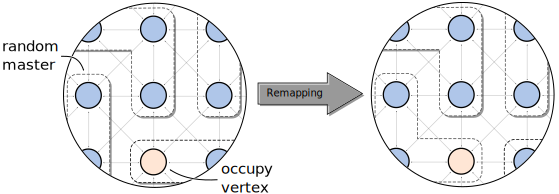
\includegraphics[width=\textwidth]{graphics/40_gol_remapping}
    \caption{Remapping of vertices to peers. A random master host is
      determined by a consensus random number generation. The master
      dictates the vertex which will be occupied. Hosted vertices of the
      graph are reannounced.}
    \label{fig:gol_remapping}
  \end{figure}

\noindent Even though this occupation scenario is a simple example, it
shows remapping of vertices at run-time and, therefore, the potential
to establish load balancing and fault tolerance techniques on top of
the system. Ideas on load balancing and fault tolerance are discussed
in Section~\ref{sec:futurework}.
% Mehr auf load balancing und fault tolerance eingehen

\cleardoublepage

%%% Local Variables:
%%% TeX-master: "diplom"
%%% End:
